
\chapter{Electrical activity in the brain}

In this chapter we are going to discuss ...

\section{Source of the electrical activity}
\label{sec:neuron}

As all known living organisms are composed of cells, so are humans and the human brain. The brain consists of nerve cells and non-neural cells, called neurons and glial cells respectively. There are approximately 86 billion neurons in the human brain and roughly as much non-neural cells \cite{neuroncount}. A typical neuron has a cell body, multiple nerve endings, or dendrites, and one nerve fibre, or axon. Both, dendrites and axons can branch multiple times, but axons can be much longer than dendrites. 

There are connections between neurons, through which neurons can interact with each other by sending electro-chemical signals. These connections are not static and can change over time. Functionally related neurons are connected to each other and form neural pathways \cite{neuralpathway}. The general rule is that a neuron sends signals through its axon and receives signals through dendrites. The connection between an axon and a dendrite is called a synapse. See figure \ref{fig:synapse} for an example of a neuron and a synapse.

\begin{figure}[b!]
	\begin{minipage}{0.5\textwidth}
		\centering
		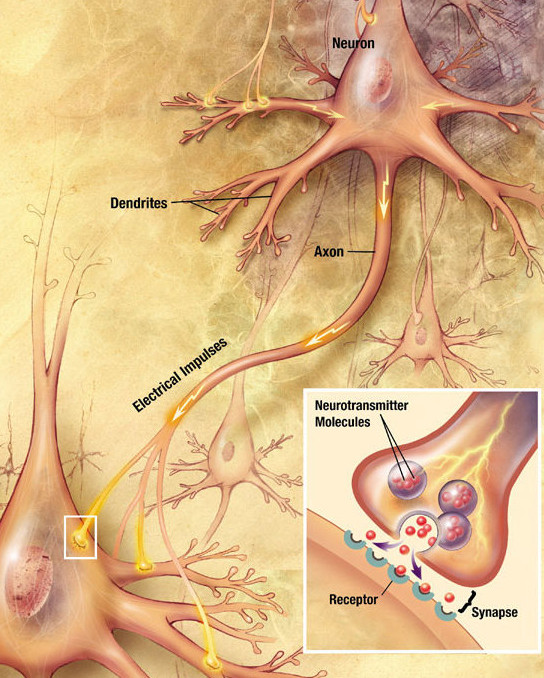
\includegraphics[width=\textwidth]{synapse.jpg}
		\caption{Neurons and chemical synapse \cite[p.~17]{neuronpic}}
		\label{fig:synapse}
	\end{minipage}
	\begin{minipage}{0.5\textwidth}
		\centering
		%\includegraphics[width=\textwidth]{ActionPotential.png}
		\caption{Resting and action potential}
		\label{fig:action_potential}
	\end{minipage}
\end{figure}

To send signals, neurons must be able to maintain electrical potential, called membrane potential. Membrane potential is the difference in electric potential between the interior and exterior of a cell. When neurons are not sending signals, they have slightly negative membrane potential which is called resting potential. Negative resting potential is achieved by having more positively charged ions inside the cell than around it.

By having stable resting potential, neuron is able to send signals by rapidly increasing and decreasing the membrane potential along an axon. Therefore, the signal travelling along an axon is actually higher membrane potential. This event is called an action potential. To increase or decrease the membrane potential of a cell, ionophoric proteins are used. These proteins transport ions across the cell membrane.

Action potential is initiated by a certain threshold voltage, called threshold potential. When the membrane potential of a neuron exceeds threshold potential, the neuron sends signals to other cells. The neuron that receives the signal is called postsynaptic cell. Synaptic input in a postsynaptic cell can cause the membrane potential of the postsynaptic terminal to increase or decrease. These events are called postsynaptic potentials.

Postsynaptic potentials cause small electric currents. When ions start entering the cell near postsynaptic terminal, the concentration of these ions increase in this location and they start to move along a dendrite towards cell body. This movement generates current dipole.

\section{Functional neuroimaging}
\label{sec:neuroimaging}

As discussed in section \ref{sec:neuron}, neurons in the brain are sending electrochemical signals to communicate with each other. There are several techniques available to measure this activity and before we continue to discuss the biological background we will be giving a brief overview of these methods. Measuring an aspect of brain function is called functional neuroimaging and common measurement methods divide into haemodynamic and electromagnetic techniques.

Haemodynamic techniques measure blood oxygenation and blood flow in the brain. More oxygen has to be delivered to more active brain regions and this allows the brain activity to be measured. Haemodynamic techniques include functional \acrfull{fMRI}, \acrfull{fNIRS}, \acrfull{PET}.

Electromagnetic techniques measure either electrical activity or magnetic fields produced by the electrical activity along the scalp. Electromagnetic techniques include \acrfull{EEG} and \acrfull{MEG}. These methods have lower temporal resolution than haemodynamic methods, but measure only the activity in the outer layer of the brain. Temporal resolution is the smallest time period of neural activity that is reliably separated out by measuring technique.
%http://psychcentral.com/lib/types-of-brain-imaging-techniques/0001057
%http://www.macalester.edu/academics/psychology/whathap/UBNRP/Imaging/eeg.html
%http://scienceforthemasses.org/2014/04/11/selecting-an-eeg-device/

To decide which method is best for controlling a robot, we will compare cost, portability and temporal resolution of each method. See table \ref{tab:neuroimaging} for details. For real time robot controlling, lower temporal resolution is better, because it enables faster decision making. We also prefer techniques that are portable and available for the consumer, so the usage would not be limited to certain location and would be available to the people in need. Considering all these arguments, it can be seen that the best choice for controlling a robot is an \acrshort{EEG} device.

% Constants for table

\newcommand{\pMEG}{\tablefootnote{http://neurogadget.com/2012/12/15/inexpensive-magnetoencephalography-meg-system-could-be-available-at-every-hospital/6495}}
\newcommand{\pfMRI}{\tablefootnote{http://info.blockimaging.com/bid/92623/MRI-Machine-Cost-and-Price-Guide}}
\newcommand{\pPET}{\tablefootnote{http://info.blockimaging.com/bid/68875/How-Much-Does-a-PET-CT-Scanner-Cost}}
\newcommand{\plEEG}{\tablefootnote{http://en.wikipedia.org/wiki/Comparison\_of\_consumer\_brain-computer\_interfaces}}
\newcommand{\phEEG}{\tablefootnote{http://www.brainvision.com/files/actiCHamp-PyCorder-Flyer\_US.pdf}}
\newcommand{\pNIRS}{\cite{NIRS}}
\newcommand{\tresol}{\cite{timeresol}}

% Table

\begin{table}[h]
	\centering
	\begin{tabular}{|c|c|c|c|c|c|}
	\hline
				& Price	from				& Portable	& Temporal resolution	& Special requirements		\\\hline
\acrshort{MEG}	& millions\pMEG				& no	& milliseconds \tresol		& magnetically shielded room\\\hline
\acrshort{fMRI}	& \SI{150000}[\$]\pfMRI		& no	& about 1 second \tresol	& magnetically shielded room\\\hline
\acrshort{PET}	& \SI{125000}[\$]\pPET		& no	& about 1 second \tresol	& radioactive isotopes injection\\\hline
\acrshort{fNIRS}& \SI{10000}[\$]{} \pNIRS	& yes	& hundreds of milliseconds \pNIRS&						\\\hline
\acrshort{EEG}	& \SI{100}[\$]\plEEG		& yes	& milliseconds \tresol		&							\\\hline
	\end{tabular}
	\caption{Comparison of functional neuroimaging methods}
	\label{tab:neuroimaging}
\end{table}

\section{Electroencephalography}

As already mentioned in the previous section, \acrshort{EEG} measures the electrical activity along the scalp. This electrical activity originates from the communication between neurons, as discussed in section \ref{sec:neuron}. However, the electric potential generated by one neuron is far too low to be recognized. Therefore, thousands or millions of neurons have to 

%Oscillatory activity can also be used to control external devices in brain?computer interfaces, in which subjects can control an external device by changing the amplitude of particular brain rhythmics. (http://en.wikipedia.org/wiki/Neural_oscillation)
\section{Visual evoked potential}

\section{Emotiv EPOC}
In section \ref{sec:neuroimaging} we briefly compared different functional neuroimaging methods and concluded that currently \acrshort{EEG} is most suitable for our needs. But there is a wide variety of EEG devices available. 
 